\section{Models of FIFOs}
\label{sec:model:fifos}
This section presents the automata corresponding to message FIFOs. Having the
FIFOs kept separate from the components greatly simplifies the components'
automata. Indeed, it would otherwise be needed for every state of the
components' automata to be ready for a synchronization related to message
exchanges. Instead, two very similar automata are used, both having an incoming
and outgoing message queue. The automata are given the component ID of the
component they act for, instead of a dedicated one.

\subsection{Query FIFO}
\begin{figure}[hbt!]
\begin{center}
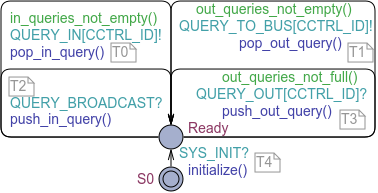
\includegraphics[width=0.5\textwidth]{\chapterdirectory/figure/QueryFIFO.pdf}
\end{center}
\caption{Automaton for a Query FIFO}
\label{fig:UPPAAL:QueryFIFO}
\end{figure}

Figure~\ref{fig:UPPAAL:QueryFIFO} shows the automaton for transfer of queries.
It simply maintains two arrays of queries with first-in-first-out access
policies. These two arrays are the variables defined as follows:
\paragraph{Clocks \& Variables for Query FIFO}
\begin{itemize}
\item
   \lstinline!in_queries! is an array of \lstinline!IN_QUERY_BUFFER_SIZE!
   useable slots, which contains incoming query messages, and is
   maintained in a FIFO order.
\item
   \lstinline!out_queries! is an array of \lstinline!OUT_QUERY_BUFFER_SIZE!
   useable slots. It stores outgoing query messages in a FIFO order.
\end{itemize}
%\end{varandclocks}

The Query FIFO automaton starts in the $S_0$ location, wherein it awaits a
broadcast on the \textbf{SYS\_INIT}.

\paragraph{Transitions for Query FIFO}
\begin{description}
\item[$S_0 \automatatransitiontrace{T_{4}}{} \texttt{Ready}$]
   Upon synchronization on the \textbf{SYS\_INIT}, both \lstinline!in_queries!
   and \lstinline!out_queries! have their slots set to a default value which
   indicates that the slot is available.

\item[$\texttt{Ready} \automatatransitiontrace{T_{3}}{} \texttt{Ready}$]
   If \lstinline!out_queries! has available spots, the cache associated with
   this query FIFO can synchronize on the \textbf{QUERY\_OUT} sub-channel
   corresponding to the cache's component ID. This transition will retrieve
   the query that the cache put in the information sharing global variable and
   insert it at the back of the \lstinline!out_queries! queue. In addition,
   the slot of the \lstinline!has_use_for_bus! global variable corresponding to
   the cache's component ID is set to \lstinline!true!, allowing the query bus
   to know that this FIFO has content to send.

\item[$\texttt{Ready} \automatatransitiontrace{T_{1}}{} \texttt{Ready}$]
   If \lstinline!out_queries! is not empty, the automaton synchronizes with
   the query bus using the \textbf{QUERY\_TO\_BUS} sub-channel corresponding
   to the cache's component ID. The query bus will only allow the
   synchronization if this FIFO is the current bus master. This transition
   removes the oldest element of \lstinline!out_queries! and puts it in the
   information sharing global variable to communicate it to the bus.

\item[$\texttt{Ready} \automatatransitiontrace{T_{2}}{} \texttt{Ready}$]
   One would expect to see a \lstinline!in_queries_not_full()! guard on this
   transition, however, the \textbf{QUERY\_BROADCAST} channel is set to
   broadcast, meaning that preventing this transition from firing does not
   prevent the broadcast from being made. Thus, it would lead to the query never
   being received by this FIFO. Instead, the \lstinline!is_ready_for_bus!
   global variable is used to ensure that all components that need to see
   queries are ready. Thus, if the transition occurs, the \lstinline!in_queries!
   queue is sure not to be full.

   Upon synchronization on the \textbf{QUERY\_BROADCAST} channel, the query held
   in the information sharing global variable is copied to the back of the
   \lstinline!in_queries! queue. In addition, the slot of the
   \lstinline!is_ready_for_bus! global variable allocated to this FIFO's
   component's ID is set to \lstinline!true! if \lstinline!in_queries! is not
   full, and to \lstinline!false! otherwise.

\item[$\texttt{Ready} \automatatransitiontrace{T_{0}}{} \texttt{Ready}$]
   If the \lstinline!in_queries! queue is not empty, synchronization on the
   \textbf{QUERY\_IN} sub-channel corresponding to this FIFO's component's ID
   leads to the oldest element of \lstinline!in_queries! being removed and
   placed in the information sharing global variable. Furthermore,
   the \lstinline!is_ready_for_bus! slot relevant for this FIFO is set to
   \lstinline!true!, as a free spot has just been created.
\end{description}

\subsection{Data FIFO}
\begin{figure}[hbt!]
\begin{center}
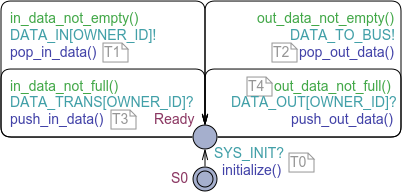
\includegraphics[width=0.5\textwidth]{\chapterdirectory/figure/DataFIFO.pdf}
\end{center}
\caption{Automaton for a Data FIFO}
\label{fig:UPPAAL:DataFIFO}
\end{figure}

Figure~\ref{fig:UPPAAL:DataFIFO} shows the automaton corresponding to a Data
FIFO. It works like the one for the queries, but is simpler, as it does not have
to handle any broadcast synchronizations. Thus, there is no need to handle
\lstinline!is_ready_for_bus! updates. These two arrays variables are thus also
present, but defined as follows:
\paragraph{Clocks \& Variables for Data FIFO}
\begin{itemize}
\item
   \lstinline!in_data! is an array of \lstinline!IN_DATA_BUFFER_SIZE!
   useable slots, which contains incoming data messages, and is
   maintained in a FIFO order.
\item
   \lstinline!out_data! is an array of \lstinline!OUT_DATA_BUFFER_SIZE!
   useable slots. It stores outgoing data messages in a FIFO order.
\end{itemize}
%\end{varandclocks}

\paragraph{Transitions for Data FIFO}
\begin{description}
\item[$S_0 \automatatransitiontrace{T_{0}}{} \texttt{Ready}$]
   Upon synchronization on the \textbf{SYS\_INIT} broadcast channel, both
   \lstinline!in_data! and \lstinline!out_data! have their slots set to a
   default value which indicates that the slot is available.

\item[$\texttt{Ready} \automatatransitiontrace{T_{4}}{} \texttt{Ready}$]
   If \lstinline!out_data! has available spots, the component associated with
   this data FIFO can synchronize on the \textbf{DATA\_OUT} sub-channel
   corresponding to the component's ID. This transition will retrieve
   the data message that the component put in the information sharing global
   variable and insert it at the back of the \lstinline!out_data! queue.

\item[$\texttt{Ready} \automatatransitiontrace{T_{2}}{} \texttt{Ready}$]
   If \lstinline!out_data! is not empty, the automaton synchronizes with the
   data bus using the \textbf{DATA\_TO\_BUS} sub-channel corresponding to this
   FIFO's component's ID. This transition removes the oldest element of
   \lstinline!out_data! and puts it in the information sharing global variable
   to communicate it to the bus.

\item[$\texttt{Ready} \automatatransitiontrace{T_{3}}{} \texttt{Ready}$]
   Since the synchronization on \textbf{DATA\_TRANS} is not a broadcast, there
   is no need for a global variable to control whether this transition can be
   fired. Instead, the guard allows the transition whenever the
   \lstinline!in_data! queue is not full. This transition takes the data message
   held in the information sharing global variable and puts it at the back of
   the \lstinline!in_data! queue.

\item[$\texttt{Ready} \automatatransitiontrace{T_{1}}{} \texttt{Ready}$]
   If the \lstinline!in_data! queue is not empty, synchronization on the
   \textbf{DATA\_IN} sub-channel corresponding to this FIFO's component's ID
   leads to the oldest element of \lstinline!in_data! being removed and
   placed in the information sharing global variable.
\end{description}
